%\PassOptionsToPackage{dvipsnames}{xcolor}
\PassOptionsToPackage{table}{xcolor} %vv important to do it this way (and not like the website says to do)!!!!
\newcommand\hmmax{0} %to deal with various fonts,e.g. mathbf
\newcommand\bmmax{0} %same
\documentclass[10pt]{beamer}

\usetheme[progressbar=frametitle]{metropolis}
\usepackage{appendixnumberbeamer}
%\setbeamersize{text margin left=5mm,text margin right=5mm} 

\usepackage{booktabs}
\usepackage[scale=2]{ccicons}

\usepackage{pgfplots}
\usepgfplotslibrary{dateplot}

\usepackage{xspace}

%\usepackage{setspace} pose problems with footnotes
\newcommand{\themename}{\textbf{\textsc{metropolis}}\xspace}

\usepackage{dashbox}
\usepackage{centernot}
\usepackage{amsmath}
\usepackage[compatibility=false]{caption}
\usepackage{wasysym}
\usepackage{fontawesome5}
\usepackage{stmaryrd}
\usepackage{marvosym}
\usepackage{subcaption}
\usepackage{multicol}
\usepackage{graphicx}
\usepackage{tabto}
\usepackage[normalem]{ulem}
\usepackage{ragged2e}
\usepackage{multirow}
\usepackage{amssymb}
\usepackage{nicefrac}
\usepackage{pifont}
\usepackage{bm}
\usepackage{cancel}
\usepackage{tikz}
\usetikzlibrary{arrows,matrix,patterns}
\usetikzlibrary {arrows.meta}
\usepackage[style=apa, natbib, sorting=ynt]{biblatex}
\renewcommand*{\bibfont}{\scriptsize}
\addbibresource{bibliography.bib}
\usepackage{breakurl}  
\usepackage{hyperref} 
\usepackage{verbatim}

\usepackage[linguistics]{forest}
\usepackage{gb4e}

%color blind friendly
\definecolor{orange}{RGB}{213, 94, 0}
\definecolor{blue}{RGB}{0, 114, 178}
\definecolor{lightblue}{RGB}{86, 180, 233}
\definecolor{green}{RGB}{0, 158, 115}
\definecolor{red}{RGB}{204, 121, 167}
\definecolor{purple}{HTML}{9467bd}




\newcommand{\p}{\textbf{\textcolor{blue}{p}}}
\newcommand{\pplus}{\textbf{\textcolor{orange}{p$^+$}}}

\newcommand{\q}{\textbf{\textcolor{red}{q}}}
\newcommand{\qplus}{\textbf{\textcolor{green}{q$^+$}}}

\newcommand{\s}{\textbf{\textcolor{pink}{s}}}
\newcommand{\splus}{\textbf{\textcolor{cyan}{s$^+$}}}
\newcommand{\splusplus}{\textbf{\textcolor{cyan}{s$^{++}$}}}

\renewcommand{\r}{\textbf{\textcolor{brown}{r}}}

\newcommand{\stronger}[1]{\textbf{\textcolor{orange}{#1}}}
\newcommand{\weaker}[1]{\textbf{\textcolor{blue}{#1}}}
\newcommand{\good}[1]{\textbf{\textcolor{green}{#1}}}
\newcommand{\bad}[1]{\textbf{\textcolor{red}{#1}}}
\newcommand{\cmark}{\textcolor{green}{\textbf{\ding{51}}}}%
\newcommand{\xmark}{\textcolor{red}{\textbf{\ding{55}}}}%


\newcommand{\Exists}{\textcolor{blue}{\bm{\exists}}}
\newcommand{\Sbna}{\textcolor{purple}{\bm{\tilde{\exists}}}}
\newcommand{\Forall}{\textcolor{orange}{\bm{\forall}}}


\newcommand{\Paris}{\textbf{\textcolor{orange}{Paris}}}
\newcommand{\France}{\textbf{\textcolor{blue}{France}}}
\setbeamerfont{bibliography item}{size=\footnotesize}
\setbeamerfont{bibliography entry author}{size=\footnotesize}
\setbeamerfont{bibliography entry title}{size=\footnotesize}
\setbeamerfont{bibliography entry location}{size=\footnotesize}
\setbeamerfont{bibliography entry note}{size=\footnotesize}


\renewcommand{\figurename}{Fig.}


\setbeamerfont{footnote}{size=\scriptsize}



\resetcounteronoverlays{exx}
\setbeamercovered{transparent}

\renewcommand{\thefootnote}{\arabic{footnote}}
\renewcommand{\thempfootnote}{\arabic{mpfootnote}}

%\setbeamertemplate{caption}[numbered] % Ensures numbered captions
\let\oldcaption=\caption
\renewcommand{\caption}[1][]{\oldcaption{\centering #1}}
\newcommand{\footciteia}[1]{\footnote{\cite{#1}, i.a.}}
\newcommand{\citenp}[1]{\citeauthor{#1}, \citeyear{#1}}


%\usefonttheme{professionalfonts} % using non standard fonts for beamer
%\usefonttheme{serif} % default family is serif
%\usepackage{fontspec}
%\setmainfont{QTCaslan}


%\usepackage[LCYW]{fontenc}
%\renewcommand*\rmdefault{obn}

%\usepackage[OT1]{fontenc}

%\usepackage{lmodern}
%\usepackage[lining]{ibarra} %% remove option 'lining' to get oldstyle figures as default
%\usepackage{OldStandard}
%\usepackage[T1]{fontenc}



\title{
\includegraphics[height=22pt]{./O.png}ddness under Discussion}
%\titlegraphic{\includegraphics[width=2cm]{qr.png}} 

\date{July 16, 2025}
\author[shortauthor]{Adèle Hénot-Mortier}

\institute{Dissertation Defense}
%\author{Adèle Hénot-Mortier (MIT)}



\begin{document}
	\metroset{block=fill}
	
	
\usebackgroundtemplate%
{%
	\includegraphics[height=\paperwidth]{./dio\_transparent.png}%
}
\begin{frame}{}
	\maketitle
\end{frame}
\usebackgroundtemplate{}

\begin{frame}{What can make sentences bad?}
	\begin{itemize}
		\item Sentences can be syntactically ill-formed.
	\end{itemize}
	\begin{exe}
		\ex[*]{Ed told Jo that he likes \textbf{herself}.}
	\end{exe}
	\begin{itemize}
		\item Sentences can be contradictory, or tautological.
	\end{itemize}
	\begin{exe}
		\ex 
		\begin{xlist}
			\ex[\#]{It's raining and it's \textbf{not} raining.}
			\ex[\#]{It's raining or it's \textbf{not} raining.}
		\end{xlist}	
	\end{exe}
	\begin{itemize}
		\item Sentences may out-of-the-blue contradict standard assumptions or expectations.
	\end{itemize}
	\begin{exe}
		\ex[??] {Jo will bring \textbf{her alligator} to the LSA.}
	\end{exe}
\end{frame}

\begin{frame}{What is oddness?}
	\begin{itemize}
		\item Sentences sometimes feel \textbf{odd} despite being informative, and perfectly ``reasonable'' is terms of what they implicitly assume.
	\end{itemize}
	Hurford Disjunction (\textbf{HD}):\vspace{-3mm}
	\begin{exe}
		\ex[\#] {Jo studied in \Paris{} or in \France. \hfill \citep{Hurford1974}\\
		\hspace*{-12mm}Conveys: Jo studied in \France.}\label{ex:hd}
	\end{exe}
	\begin{itemize}
		\item Oddness seems to come from \textbf{how} information is provided, rather than from its content.
	\end{itemize}
\end{frame}
\begin{frame}{Redundancy}
	\begin{itemize}
		\item A prominent approach to sentences like (\ref{ex:hd}), is based on \textsc{Redundancy}.\footciteia{Grice1975,Horn1984,Meyer2013,Mayr2016,Katzir2014,Kalomoiros2024}
		\item Both disjuncts of (\ref{ex:hd}) convey the information that \textit{Jo studied in \France}.
		\item In fact, the entire disjunction is contextually equivalent to (\ref{ex:fr}), which is strictly simpler!
	\end{itemize}
	\begin{exe}
		\exr{ex:hd}[\#] {Jo studied in \Paris{} or in \France. }
		\ex[] {Jo studied \sout{in \Paris{} or} in \France.}\label{ex:fr}
	\end{exe}
\end{frame}
\begin{frame}{Where Redundancy falls short}
	\begin{itemize}
			\item Oddness can arise despite the non-existence of a simpler equally informative alternative:
		\end{itemize}
	\begin{exe}
		\ex[??] {Jo studied in \France{} or  \textbf{\textcolor{green}{the Basque country}}. \hfill \citep{Singh2008a}\\
				\hspace*{-12mm}Conveys: Jo studied in \France{} or the \textbf{Spanish \textcolor{green}{Basque country}}.}\label{ex:chd}
	\end{exe}
	\begin{itemize}
			\item Sentences that are completely isomorphic contrast in terms of oddness \citep{Mandelkern2018, Kalomoiros2024}.
	\end{itemize}
	\begin{exe}
		\ex 	Hurford Conditionals (\textbf{HC}):\label{ex:hc}
		\begin{xlist}
			\ex[] {If Jo studied in \France, she did \textbf{not} study in \Paris.\\
%			\hspace*{-12mm}Conveys: If Jo studied in \France, she studied somewhere else in France than \Paris.
}\label{ex:hc-ws}
			\ex[\#] {If Jo did \textbf{not} study in \Paris, she studied in \France.\\
%				\hspace*{-12mm}Conveys: If Jo did not study in \Paris{} she studied somewhere else outside \Paris{} than \France.
				}\label{ex:hc-sw}
		\end{xlist}
	\end{exe}

%	\begin{exe}
%			\ex 
%			\begin{xlist}
%					\ex[] {Jo studied in \France, or if not in \France, in Belgium.}
%					\ex[\#] {Jo studied in \France, or if not in Belgium, in \France.}
%				\end{xlist}
%			\ex
%			\begin{xlist}
%					\ex[] {If Jo studied in \France, he did not study in Paris.}
%					\ex[\#] {If Jo did not study in Paris, he studied in \France.}
%				\end{xlist}
%		\end{exe}
\end{frame}

\begin{frame}{A new view of (implicit) questions}
	\begin{itemize}
		\item The connecting thread of my dissertation is that many cases of oddness can be explained by considering that \textbf{a good sentence has to be a good answer to a good question} \footciteia{Lewis1988, Rooth1985, Rooth1992, Roberts1996, Katzir2015,Buring2003,Zhang2022}
		\item I formalize this longstanding intuition by proposing a \textbf{compositional model of implicit questions}, which is:
			\begin{itemize}
				\item directly sensitive to the \textbf{degree of specificity} conveyed by sentences;
				\item and constrained by generalizations of \textbf{familiar pragmatic principles}.
			\end{itemize}
		\item Under that view, assertive sentences are proposals to update beliefs, but also suggest ways to hierarchically organize such beliefs.
		\item You may see that as an \textbf{extension of Dynamic Semantics at the pragmatic/inquisitive level}.
	\end{itemize}
\end{frame}

\begin{frame}{Empirical advantages}
	\begin{itemize}
		\item Making pragmatic constraints sensitive to both sentences and their implicit questions, captures cases like (\ref{ex:hd}), (\ref{ex:chd}) and (\ref{ex:hc}), that together challenge standard \textsc{Redundancy}-based approaches to oddness.
		\item Today, I will focus on two ``Hurford'' cases: disjunctions (\ref{ex:hd}) and conditionals (\ref{ex:hc}).
	\end{itemize}
	\begin{exe}
		\exr{ex:hd}{Hurford Disjunction (\textbf{HD}):\\\# Jo studied in \Paris{} or in \France.}
		\exr{ex:hc}{Hurford Conditionals (\textbf{HC}):}
		\begin{xlist}
			\ex[] {If Jo studied in \France, she did \textbf{not} study in \Paris.}
			\ex[\#] {If Jo did \textbf{not} study in \Paris, she studied in \France.}
		\end{xlist}
	\end{exe}
\end{frame}




%\begin{frame}{A Bizarre Adventure into Pragmatic Oddness}
\begin{frame}{A Bizarre Adventure into Oddness}
	\begin{enumerate}
		\item Give some \textbf{background} on assertions and questions.
		\item Define how \textbf{implicit questions} are compositionally evoked by assertions, and show why this is an independent desideratum.
		\item Capture Hurford \textbf{Disjunctions} (\ref{ex:hd}) by rephrasing \textsc{Redundancy}.
		\item Capture Hurford \textbf{Conditionals} (\ref{ex:hc}) by rephrasing \textsc{Relevance}.
		\item Discuss how implicit questions could help \textbf{outside the domain of prototypically ``odd'' sentences}.
	\end{enumerate}
\end{frame}

\usebackgroundtemplate%
{%
	\includegraphics[height=\paperwidth]{./lisalisa\_transparent.png}%
}
\begin{frame}
	\section[Background on assertions and questions]{Background on assertions and questions}
\end{frame}

\usebackgroundtemplate{}

%\begin{frame}{Back to Redundancy}
%	\begin{itemize}
%		\item The simplest \textsc{Redundancy}-based approach to oddness deems a sentence odd, if it is contextually equivalent to one of its simplifications.
%	\end{itemize}
%	\begin{exe}
%		\ex {An LF $X$ is odd if $\exists S. \ \llbracket X \rrbracket$ $\equiv$ $\llbracket S(X) \rrbracket$, with $S$ a constituent-to-subconstituent substitution operation.}
%	\end{exe}
%	\begin{itemize}
%		\item More complex variants of \textsc{Redundancy} almost always stick an extra function in the above definition.
%	\end{itemize}
%	\begin{exe}
%		\ex {An LF $X$ is odd if $\exists \langle f, S\rangle. \  \llbracket f(X) \rrbracket$ $\equiv$ $\llbracket S(f(X)) \rrbracket$, with $S$ a constituent-to-subconstituent substitution operation and $f$ an operation on LFs (e.g. subconstituent extraction).}
%	\end{exe}
%	\begin{itemize}
%		\item In any case, these approaches play with the structure of the LF, and its meaning, potentially at the local level.
%	\end{itemize}
%\end{frame}
\begin{frame}{Assertions and questions}
	\begin{itemize}
		\item Assertions typically denotes propositions (sets of worlds).
		\item The set of worlds compatible with the premises of a conversation is called Context Set (\textbf{CS}).\footcite{Stalnaker1978}
		\item Assertions update the CS by intersection.\footciteia{Stalnaker1978,Heim1982, Heim1983a,Heim1983b}
	\end{itemize}\vspace{5mm}
	\begin{figure}[H]
		\centering
		\begin{tabular}{ccc}
			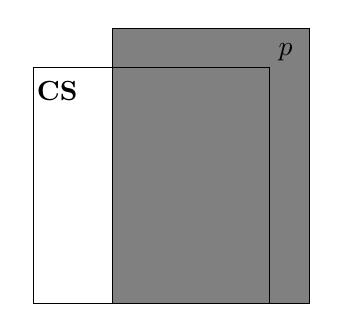
\begin{tikzpicture}
				\filldraw [draw=black,fill=gray] (1, 0) rectangle (3.5, 3.5);
				\draw [draw=black] (0, 0) rectangle (3, 3);
				\node[] (a) at (.3,2.7) {\textbf{CS}};
				\node[] (a) at (3.2,3.2) {$p$};
			\end{tikzpicture}& \begin{tabular}{c}
			$\leadsto$\\~\\~\\~\\~\\~\\
			\end{tabular} &
			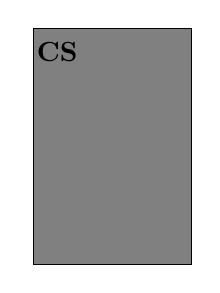
\begin{tikzpicture}
				\draw [draw=black, fill=gray] (0, 0) rectangle (2, 3);
				\node[] (a) at (.3,2.7) {\textbf{CS}};
			\end{tikzpicture}
		\end{tabular}
	\end{figure}\vspace{-2mm}
\end{frame}
\begin{frame}{Standard question semantics}
	\begin{itemize}
		\item Questions have been traditionally understood as the set of their possible answers, or ``alternatives''.\footcite{Hamblin1973,Karttunen1977}
	\end{itemize}
	\begin{exe}
		\ex {$\llbracket$Who did the readings?$\rrbracket$ = $\lbrace$Ed, Al, Ed and Al, ...$\rbrace$}
	\end{exe}
	\begin{itemize}
		\item Alternatives are not necessarily exclusive: if Ed and Al did the readings then Ed did the readings.
		\item Stronger alternatives, intuitively correspond to ``better'' answers.
		\item Given that questions are sets of propositions, how are they supposed to affect the CS?
	\end{itemize}
	
\end{frame}

\begin{frame}{Standard question pragmatics}
	\begin{itemize}
		\item Questions induce a \textbf{partition of the CS}: just group together the worlds of the CS that agree on all alternatives.\footcite{Groenendijk1984}
		\item The ``groups'' are called \textbf{cells}: they tell us which distinctions matter.
	\end{itemize}\vspace{-2mm}

	\begin{overprint}
		\onslide<1>
			\begin{figure}[H]
				\centering	\scalebox{.8}{
					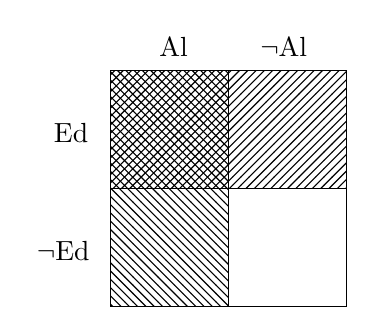
\begin{tikzpicture}	
						\node[] at(.8, 3.3) {Al};
						\node[] at(2.2, 3.3) {$\neg$Al};
						\node[] at(-.6, .7) {$\neg$Ed};
						\node[] at(-.5, 2.2) {Ed};
						\draw [draw=black] (0, 0) rectangle (3, 3);
						\draw [draw=black,pattern=north west lines] (0, 0) rectangle (1.5, 3);
						\draw [draw=black,pattern=north east lines] (0,1.5) rectangle (3, 3);
				\end{tikzpicture}}\\
				{\textbf{Step 1: }Check how each world deals with the alternatives: 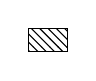
\begin{tikzpicture}
						\draw [draw=black,pattern=north west lines] (0, 0) rectangle (.5, .3);
					\end{tikzpicture} defines \textit{Al did the readings} and 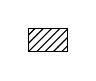
\begin{tikzpicture}
						\draw [draw=black,pattern=north east lines] (0, 0) rectangle (.5, .3);
					\end{tikzpicture} defines \textit{Ed did the readings}.}\label{fig1:alternatives}
		\end{figure}
		
		\onslide<2>
			\begin{figure}[H]
				\centering\scalebox{.8}{
					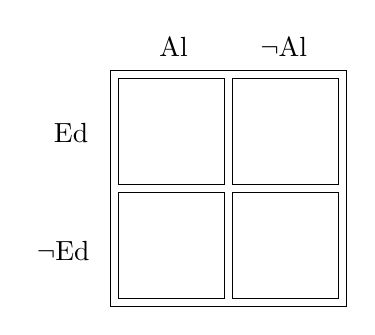
\begin{tikzpicture}	
						\node[] at(.8, 3.3) {Al};
						\node[] at(2.2, 3.3) {$\neg$Al};
						\node[] at(-.6, .7) {$\neg$Ed};
						\node[] at(-.5, 2.2) {Ed};
						\draw [draw=black] (0, 0) rectangle (3, 3);
						\draw [draw=black] (0.1, 1.55) rectangle (1.45, 2.9);
						\draw [draw=black] (1.55, 0.1) rectangle (2.9, 1.45);
						\draw [draw=black] (0.1, 0.1) rectangle (1.45, 1.45);
						\draw [draw=black] (1.55, 1.55) rectangle (2.9, 2.9);
				\end{tikzpicture}}\\
				{\textbf{Step 2: }Partition the CS by grouping worlds with the same ``pattern''. }\label{fig1:cells}
		\end{figure}
	\end{overprint}
	
	\begin{itemize}
		\item We will only consider exhaustive and mutually exclusive alternatives, s.t. question semantics and question pragmatics in fact coincide.
	\end{itemize}\vspace{3mm}
\end{frame}

\begin{frame}{Answering questions}
	\begin{itemize}
		\item Here the cells are \textit{only Ed did the readings}, \textit{only Al}, \textit{Ed an Al}, and \textit{neither}. Those are \textbf{maximal answers}.
		\item Union of cells, e.g. \textit{Ed did the readings} (including \textit{only Ed}, and \textit{both}), are \textbf{non-maximal answers}.
	\end{itemize}
	\begin{figure}[H]
		\centering\scalebox{.8}{
			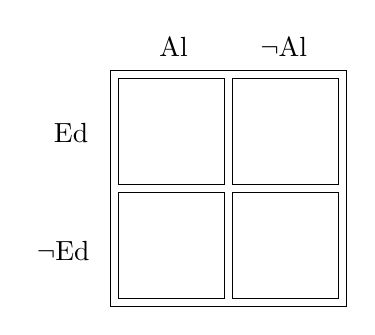
\begin{tikzpicture}	
				\node[] at(.8, 3.3) {Al};
				\node[] at(2.2, 3.3) {$\neg$Al};
				\node[] at(-.6, .7) {$\neg$Ed};
				\node[] at(-.5, 2.2) {Ed};
				\draw [draw=black] (0, 0) rectangle (3, 3);
				\draw [draw=black] (0.1, 1.55) rectangle (1.45, 2.9);
				\draw [draw=black] (1.55, 0.1) rectangle (2.9, 1.45);
				\draw [draw=black] (0.1, 0.1) rectangle (1.45, 1.45);
				\draw [draw=black] (1.55, 1.55) rectangle (2.9, 2.9);
		\end{tikzpicture}}
		\end{figure}
		\begin{itemize}
			\item Questions \textit{encode} maximal answers only. The non-maximal ones can be \textit{derived} by union. 
		\end{itemize}
\end{frame}
\begin{frame}{Constraints on question-answer pairs: Congruence}
	\begin{itemize}
		\item It is widely accepted that the pairs formed by overt questions and answers are subject to constraints.
		\item On the semantic side, answer better be ``congruent'' with the question. This explains the pattern in (\ref{ex:congruence}).
	\end{itemize}
	\begin{exe}
		\ex {\textsc{Question-Answer Congruence} (\citet{Rooth1992}'s version). For a pair $\langle Q, A \rangle$ to be well-formed, any alternative in $\llbracket Q \rrbracket$, must be obtainable from a substitution of $A$'s focused material.}\label{ex:qa-congruence}
	\end{exe}
	\begin{exe}
		\ex {Who did the readings?
		}\label{ex:congruence}
		\begin{xlist}
			\ex[] {ED did the readings.}
			\ex[\#] {Ed did the READINGS.}
		\end{xlist}
	\end{exe}
\end{frame}

\begin{frame}{Constraints on question-answer pairs: Relevance}
	\begin{itemize}
		\item Another constraint is \textsc{Relevance}, and spells out the intuition that questions drive what sort of information their answer should convey.
		\begin{exe}
			\ex {\textsc{Relevance} (\citet{Kriz2020}'s version). An answer is relevant to a question if it corresponds to a non-maximal union of cells.}
		\end{exe}
		\item The idea that similar constraints are at play beyond overt QA pairs, has been around for a while,\footciteia{Lewis1988,Roberts1996,Riester2019} but the systematic link between assertions and questions is still poorly understood.
	\end{itemize}
\end{frame}
\begin{frame}{Preview: Oddness as question-answer Incongruence}
	\begin{itemize}
		\item Recall oddness seems to arise from how information is conveyed, rather than from its content.
		\item I submit that this ``how'' it tied to which question we are trying to address.
		\item Oddness then arises from the interaction between assertions and the (implicit) question(s) they are trying to address.
		\item \textbf{An odd sentence is a sentence that only gives rise to odd questions.}
	\end{itemize}
\end{frame}


\usebackgroundtemplate%
{%
		\includegraphics[height=\paperwidth]{./josuke\_transparent.png}%
	}
\begin{frame}
	\section[Compositional Implicit Questions]{Compositional Implicit Questions}
\end{frame}
\usebackgroundtemplate{}


\begin{frame}{Constraining assertions and  their implicit questions}
	\begin{itemize}
		\item If odd sentence gives rise to odd questions, then \textbf{the pragmatic module must then be sensitive to pairs formed by sentences and their implicit questions.}
		\item Oddness then arises when none of the implicit questions evoked by a sentence, is felicitous, given that sentence.
	\end{itemize}
	\begin{center}
		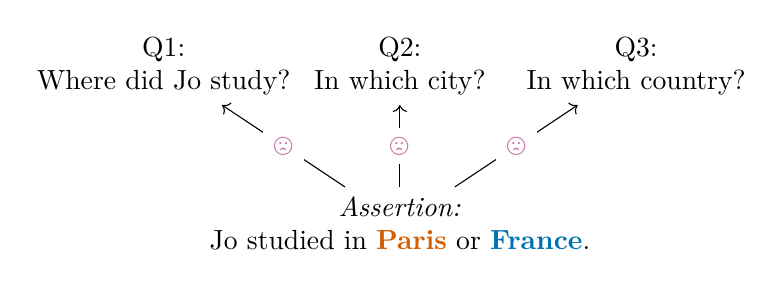
\begin{tikzpicture}
			\node[align=center] at(0, 0) (A) {\textit{Assertion:}\\ Jo studied in \Paris{} or \France.};
			\node[align=center] at(-3, 2) (Q1) {Q1:\\ Where did Jo study?};
			\node[align=center] at(0, 2) (Q2) {Q2:\\ In which city?};
			\node[align=center] at(3, 2) (Q3) {Q3:\\ In which country?};
			\draw[->] (A) -- (Q1) node[midway, fill=white] {\textcolor{red}{\frownie}};
			\draw[->] (A) -- (Q2) node[midway, fill=white] {\textcolor{red}{\frownie}};
			\draw[->] (A) -- (Q3) node[midway, fill=white] {\textcolor{red}{\frownie}};
		\end{tikzpicture}
	\end{center}
\end{frame}

\begin{frame}{A desideratum to guide our framework}
	\begin{itemize}
		\item Assertions should evoke questions matching their level of specificity. This is obviously supported by overt QA pairs:
	\end{itemize}
	\begin{exe}
		\ex \label{ex:qa-gran}
		\begin{xlist}
			\ex {Where did Jo study? --$\lbrace$\Paris, \France$\rbrace$.}
			\ex {In which country did Jo study? --$\lbrace$\#\Paris, \France$\rbrace$}
			\ex {In which city did Jo study? --$\lbrace$\Paris, \#\France$\rbrace$}
		\end{xlist}
	\end{exe}
	\begin{itemize}
		\item Basic alternative semantics does not fully capture this: generating a question from a proposition by replacing its focused material with same-type alternatives does not guarantee that the outputs will have same specificity.\footnote{Assuming alternatives must be ``relevant'' does not really help either: one must then explain how relevance incorporates specificity.}
		\item As a result, the evoked question may mix alternatives like \Paris{} and \France, giving rise to weird partitions.
	\end{itemize}\vspace{2mm}
\end{frame}

\begin{frame}{Additional motivations for a specificity constraint}
	\begin{itemize}
		\item Does question-answer \textsc{Relevance} help achieve the specificity desideratum? Not quite: both answer in (\ref{ex:qa-gran2}) are unions of cells and as such \textsc{Relevant}, yet (\ref{ex:qa-gran2-c}) feels too-coarse grained.
	\end{itemize}
	\begin{exe}
		\ex {In which country did Jo study?}\label{ex:qa-gran2}
		\begin{xlist}
			\ex[\#] {\textbf{\textcolor{green}{Western Europe}}}\label{ex:qa-gran2-c}
			\ex[]  {\France, \textbf{\textcolor{blue}{the UK}}, or \textbf{\textcolor{blue}{Germany}}}\label{ex:qa-gran2-f}
		\end{xlist}
	\end{exe}
	\begin{itemize}
		\item Intuitively, (\ref{ex:qa-gran2-c}) evokes a \textit{which area} question while (\ref{ex:qa-gran2-f}) evokes a \textit{which country} question, and the former is coarser-grained than the latter.
		\item \textbf{We need a model of questions that encodes specificity relations between propositions -- and questions themselves.}
	\end{itemize}
\end{frame}





\begin{frame}{Questions as nested partition}
		\begin{itemize}
			\item Question are modeled as \textbf{nested} partitions. Nesting is based on specificity:\footnote{Specificity is formalized in the dissertation using Hasse diagrams for $\vDash$ defined on complete sets of alternatives.} nested partitions are finer-grained than nesting partitions, meaning, \Paris{} and \France{} cannot be mixed up.
			\item A ``fine-grained'' question may then contain coarser-grained questions, meaning, a \textit{which city} question structurally refines a \textit{which country} question.
		\end{itemize}
		\begin{figure}[H]
			\centering
			\begin{subfigure}[t]{.3\linewidth}
				\centering
				\scalebox{.7}{
					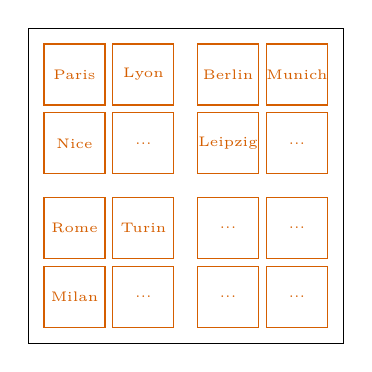
\begin{tikzpicture}	
						\draw [draw=black] (0, 0) rectangle (4,4) ;
						\draw [draw=orange] (0.2, 2.15) rectangle (0.975, 2.925) node[pos=.5] {\tiny \textcolor{orange}{Nice}};
						\draw [draw=orange] (1.075, 2.15) rectangle (1.85, 2.925) node[pos=.5] {\tiny \textcolor{orange}{...}};
						\draw [draw=orange] (0.2, 3.025) rectangle (0.975, 3.8) node[pos=.5] {\tiny \textcolor{orange}{Paris}};
						\draw [draw=orange] (1.075, 3.025) rectangle (1.85, 3.8) node[pos=.5] {\tiny \textcolor{orange}{Lyon}};
						\draw [draw=orange] (0.2, 0.2) rectangle (0.975, 0.975) node[pos=.5] {\tiny \textcolor{orange}{Milan}};
						\draw [draw=orange] (1.075, 0.2) rectangle (1.85, 0.975) node[pos=.5] {\tiny \textcolor{orange}{...}};
						\draw [draw=orange] (0.2, 1.075) rectangle (0.975, 1.85) node[pos=.5] {\tiny \textcolor{orange}{Rome}};
						\draw [draw=orange] (1.075, 1.075) rectangle (1.85, 1.85) node[pos=.5] {\tiny \textcolor{orange}{Turin}};
						
						\draw [draw=orange] (2.15, 0.2) rectangle (2.925, 0.975) node[pos=.5] {\tiny \textcolor{orange}{...}};
						\draw [draw=orange] (3.025, 0.2) rectangle (3.8, 0.975) node[pos=.5] {\tiny \textcolor{orange}{...}};
						\draw [draw=orange] (2.15, 1.075) rectangle (2.925, 1.85) node[pos=.5] {\tiny \textcolor{orange}{...}};
						\draw [draw=orange] (3.025, 1.075) rectangle (3.8, 1.85) node[pos=.5] {\tiny \textcolor{orange}{...}};
						
						\draw [draw=orange] (2.15, 2.15) rectangle (2.925, 2.925) node[pos=.5] {\tiny \textcolor{orange}{Leipzig}};
						\draw [draw=orange] (3.025, 2.15) rectangle (3.8, 2.925) node[pos=.5] {\tiny \textcolor{orange}{...}};
						\draw [draw=orange] (2.15, 3.025) rectangle (2.925, 3.8) node[pos=.5] {\tiny \textcolor{orange}{Berlin}};
						\draw [draw=orange] (3.025, 3.025) rectangle (3.8, 3.8) node[pos=.5] {\tiny \textcolor{orange}{Munich}};
				\end{tikzpicture}}
				\caption{By-city partition.}\label{fig2:city-partition}
			\end{subfigure}\hfill
			\begin{subfigure}[t]{.3\linewidth}
				\centering
				\scalebox{.7}{
					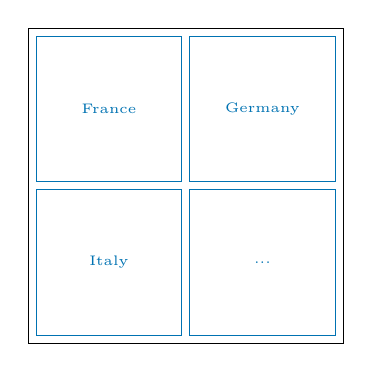
\begin{tikzpicture}	
						\draw [draw=black] (0, 0) rectangle (4,4);
						\draw [draw=blue] (0.1, 2.05) rectangle (1.95, 3.9) node[pos=.5] {\tiny \textcolor{blue}{France}};
						\draw [draw=blue] (2.05, 0.1) rectangle (3.9, 1.95) node[pos=.5] {\tiny \textcolor{blue}{...}};
						\draw [draw=blue] (0.1, 0.1) rectangle (1.95, 1.95) node[pos=.5] {\tiny \textcolor{blue}{Italy}};
						\draw [draw=blue] (2.05, 2.05) rectangle (3.9, 3.9) node[pos=.5] {\tiny \textcolor{blue}{Germany}};
				\end{tikzpicture}}
				\caption{By-country partition}\label{fig2:country-partition}
			\end{subfigure}\hfill
			\begin{subfigure}[t]{.3\linewidth}
				\centering				\scalebox{.7}{
				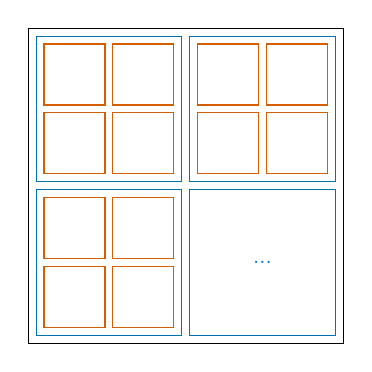
\begin{tikzpicture}	
					\draw [draw=black] (0, 0) rectangle (4,4) ;
					\draw [draw=blue] (0.1, 2.05) rectangle (1.95, 3.9);
					\draw [draw=orange] (0.2, 2.15) rectangle (0.975, 2.925);
					\draw [draw=orange] (1.075, 2.15) rectangle (1.85, 2.925);
					\draw [draw=orange] (0.2, 3.025) rectangle (0.975, 3.8);
					\draw [draw=orange] (1.075, 3.025) rectangle (1.85, 3.8);
					\draw [draw=blue] (2.05, 0.1) rectangle (3.9, 1.95) node[pos=.5] {\scriptsize \textcolor{blue}{...}};
					\draw [draw=blue] (0.1, 0.1) rectangle (1.95, 1.95);
					\draw [draw=orange] (0.2, 0.2) rectangle (0.975, 0.975);
					\draw [draw=orange] (1.075, 0.2) rectangle (1.85, 0.975);
					\draw [draw=orange] (0.2, 1.075) rectangle (0.975, 1.85);
					\draw [draw=orange] (1.075, 1.075) rectangle (1.85, 1.85);
					\draw [draw=blue] (2.05, 2.05) rectangle (3.9, 3.9);
					\draw [draw=orange] (2.15, 2.15) rectangle (2.925, 2.925);
					\draw [draw=orange] (3.025, 2.15) rectangle (3.8, 2.925);
					\draw [draw=orange] (2.15, 3.025) rectangle (2.925, 3.8);
					\draw [draw=orange] (3.025, 3.025) rectangle (3.8, 3.8);
				\end{tikzpicture}}
				\caption{Recursive partition.}\label{fig2:city-recursive-partition}
			\end{subfigure}
		\end{figure}
\end{frame}

\begin{frame}{Useful notational variant: questions as Trees}
	\begin{itemize}
		\item  Nested partitions will be represented as \textbf{trees}. The layers of a question-tree have same specificity.
		\item Simplex sentences like \textit{Jo studied in \Paris} may then evoke nested ``\textit{wh}'' questions-trees like \ref{fig:qtree-paris-wh}, or polar question trees like \ref{fig:qtree-paris-polar}.
		\item \textbf{Their deepest layers matches the prejacent's specificity.}\footnote{This recipe already get us the challenging ``compatible'' Hurford cases like (\ref{ex:chd}), (almost) for free!}
	\end{itemize}
	\begin{figure}[H]
		\centering
		\begin{subfigure}[b]{.6\linewidth}
			\centering\scalebox{.8}{
			\begin{forest}
				[{Context Set (\textbf{CS})}[Europe[\France[\Paris][\stronger{...}]][\weaker{Italy}[\stronger{...},roof]][\weaker{...}]][Asia[\weaker{...},roof]][...]]
			\end{forest}}
			\caption{``\textit{Wh}'' tree}\label{fig:qtree-paris-wh}
		\end{subfigure}\hfill	
		\begin{subfigure}[b]{.35\linewidth}
			\centering		\scalebox{.9}{
			\begin{forest}
				[CS[\Paris][not \Paris]]
			\end{forest}}
			\caption{``Polar'' tree}\label{fig:qtree-paris-polar}
		\end{subfigure}\vspace{-3mm}
		\caption{Trees evoked by \textit{Jo studied in \Paris}.}
	\end{figure}
\end{frame}
\begin{frame}{Benefits of trees beyond specificity encoding}
	\begin{itemize}
		\item Implicit questions\footcite{Carlson1985,vonStutterheim1989,vanKuppevelt1995a,vanKuppevelt1995b,Ginzburg1996,Ginzburg2012}, and question trees\footciteia{Roberts1996,Buring2003,Riester2019,Onea2016,Zhang2022,Ippolito2019} have been around for a while. \citet{Ippolito2019} even discussed how specificity differences in trees could capture oddness.
		\item But none of the previous approaches leveraged the expressivity of a tree model, to render the idea that \textbf{the questions evoked by a sentence, are compositionally derived from its LF}.
		\item This is needed if one wants to make precise predictions about logically similar, but structurally different sentences, like Hurford Conditionals.
		\item We now introduce a set of rules for $\neg$, $\vee$, and conditionals, that apply to trees and \textbf{recycle longstanding intuitions about these operators.}
	\end{itemize}\vspace{2mm}
\end{frame}


\begin{frame}{Flagging, and ``negating'' Questions Trees}
	\begin{itemize}
		\onslide<1>{\item When a simple assertion evokes an implicit question tree, leaves entailing the assertion get flagged; \textbf{flags track ``at-issue'' meaning, and are compositionally derived}.}
		\onslide<2>{\item Negating an assertion \textbf{flips the flags} on this assertion's trees. Flag-flipping is a layerwise \textbf{complement set} operation.}
	\end{itemize}
	\begin{overprint}
	\onslide<1>
		\begin{figure}[H]
			\centering
			\scalebox{.85}{
				\begin{forest}
					[CS[Europe[\France[{\faFlagCheckered\\\Paris}][{\stronger{Lyon}}][{\stronger{...}}]][\weaker{Italy}[{\stronger{...}},roof]][\weaker{...}]][Asia[\weaker{...},roof]][...]]
			\end{forest}}
		\caption{A tree for \textit{Jo studied in \Paris.}}
		\end{figure}
	
	
	\onslide<2>
		\begin{figure}[H]
			\centering
			\scalebox{.85}{
				\begin{forest}
					[CS[Europe[\France[{\Paris}][{\faFlagCheckered\\\stronger{Lyon}}][{\faFlagCheckered\\\stronger{...}}]][\weaker{Italy}[{\faFlagCheckered\\\stronger{...}},roof]][\weaker{...}]][Asia[\weaker{...},roof]][...]]
			\end{forest}}
			\caption{A tree for \textit{Jo did \textbf{not} study in \Paris.}}
		\end{figure}	
	
	\end{overprint}
\end{frame}

\begin{frame}{Disjoining Questions Trees}
	\begin{itemize}
		\item Disjunction fuses the trees evoked by the disjuncts, retaining only unions that are well-formed nested partitions.
		\item Set of flagged nodes are also merged.
	\end{itemize}
	\begin{minipage}{.45\linewidth}
		\centering
		\begin{figure}[H]
			\centering
			\scalebox{.7}{
				\begin{forest}
					[CS[\France[{\faFlagCheckered\\\Paris}][\stronger{Lyon}][\stronger{...}]][\weaker{Italy}[\stronger{...},roof]][\weaker{...}]]
			\end{forest}}\vspace{-3mm}
		\caption{A tree for \textit{Jo studied in \Paris}.}
		\end{figure}
	\end{minipage}
	\hfill
	\begin{minipage}{.05\linewidth}
		\centering
		{\LARGE $\cup$}\\~\\
	\end{minipage}
	\hfill
	\begin{minipage}{.45\linewidth}
		\centering
		\begin{figure}[H]
			\centering
			\scalebox{.7}{
				\begin{forest}
					[CS[\faFlagCheckered\\\France][\weaker{Italy}][\weaker{...}]]
			\end{forest}}\vspace{-3mm}
			\caption{A tree for \textit{Jo studied in \France}.}
		\end{figure}
	\end{minipage}
	
	\begin{center}
		\vspace{-8mm}
		\begin{minipage}{.05\linewidth}
		\centering
		{\LARGE =}
	\end{minipage}
	\begin{minipage}{.7\linewidth}
		\begin{figure}[H]
			\scalebox{.7}{
				\begin{forest}
					[CS[{\faFlagCheckered\\\France}[{\faFlagCheckered\\\Paris}][\stronger{Lyon}][...]][\weaker{Italy}[\stronger{...},roof]][\weaker{...}]]
			\end{forest}}\vspace{-3mm}
		\caption{A tree for \#\textit{Jo studied in \Paris{} or \France}.}
		\end{figure}
	\end{minipage}
	\end{center}

\end{frame}

\begin{frame}{Conditional Questions Trees}
	\begin{minipage}{.55\linewidth}
		\begin{itemize}
			\item Conditional are often taken to \textbf{restrict the evaluation of the consequent} to the worlds in which the antecedent holds.\footciteia{Lewis1975,Heim1982,Kratzer1986,Kratzer1991}
			\item Therefore, we assume that conditional question-trees raise a question evoked by the consequent, only where the antecedent holds.
			\item Technically, conditionals \textbf{``plug'' consequent trees, into the flagged leaves of the antecedent trees} -- keeping only the consequent's flags.
		\end{itemize}
	\end{minipage}\hfill
	\begin{minipage}{.4\linewidth}
		\centering
		\begin{figure}[H]
			\centering
			\begin{minipage}{\linewidth}
				\centering
				\scalebox{.8}{
					\begin{forest}
						[CS[\xcancel{\faFlagCheckered}\\\France][\weaker{Italy}][\weaker{...}]]
				\end{forest}}
			\end{minipage}
			\begin{minipage}{\linewidth}
				\centering
				\scalebox{.8}{
				\begin{forest}
					[{CS$\cap$\France}[{\stronger{Paris}}][{\faFlagCheckered\\\stronger{Lyon}}][{\faFlagCheckered\\\stronger{...}}]]
					\draw[->] (0, .5) to[out=north, in=south] (-1, 1.2);
			\end{forest}}
		\end{minipage}\vspace{-3mm}
			\caption{A tree for \textit{If Jo studied in \France, she did \textbf{not} study in \Paris}.}
		\end{figure}
	\end{minipage}
\end{frame}

\begin{frame}{Interim Summary: expressivity}
	\begin{itemize}
		\item Questions were modeled as \textbf{nested partitions}, represented as trees. Even if they look bulkier, they are just the inductive closure of an existing, incontroversial object: partitions of the CS.
		\item Trees are expressive enough to capture the intuition that some assertions (e.g. \textit{\Paris, \stronger{London}}) are more specific than others (e.g. \textit{\France}), in that they evoke more ``ramified'' trees. \textbf{Specificity is made directly available to the pragmatic module.}
	\end{itemize}

		\begin{figure}[H]
			\centering
			\scalebox{.8}{
				\begin{forest}
					[CS[\France[{\Paris}][\stronger{Lyon}][\stronger{...}]][\weaker{Italy}[\stronger{...},roof]][\weaker{...}]]
					\draw [draw=orange] (-3.2, .7) rectangle (2, -2.7);
					\draw [draw=blue] (-2.3, .5) rectangle (1.8, -1.4);
					\draw [draw=orange] (-3.2, -2) -- (-4, -2);
					\draw [draw=blue] (-2.3, -1) -- (-4, -1);
					\node[] at(-5.4, -2) {Tree for \Paris};
					\node[] at(-5.4, -1) {Tree for \France};
			\end{forest}}
		\end{figure}
	\begin{itemize}
		\item This will be exploited in two different ways when we deal with Hurford Disjunctions and Conditionals.
	\end{itemize}
\end{frame}
\begin{frame}{Interim Summary: transparency}
	\begin{itemize}
		\item Disjunctions and conditionals can evoke different tree structures, \textit{independently of their assigned semantics}:\footnote{This makes the current approach crucially different from Inquisitive Semantics. (\citenp{Mascarenhas2008}; \citenp{Ciardelli2009}; \citenp{Groenendijk2009}; \citenp{Ciardelli2017}; \citenp{Ciardelli2018}; \citeauthor{Zhang2024}, to appear)}
		\begin{itemize}
			\item Disjunctive trees are formed with $\cup$, capturing the idea that \textbf{disjuncts answer the same global question}.\footcite{Simons2001,Zhang2022,Westera2020}
			\item Conditional trees are formed \textit{via} an asymmetric $\cap$, capturing the idea that \textbf{antecedents are restrictors}.\footcite{Lewis1975,Kratzer1986,Heim1982}
		\end{itemize}
		\item This will allow us to capture the challenging contrast in Hurford Conditionals (and the absence thereof in Disjunctions) in an intuitive way.
	\end{itemize}
\end{frame}


\usebackgroundtemplate%
{%
	\includegraphics[height=\paperwidth]{./giorno\_transparent.png}%
}
\begin{frame}
	\section[Rephrasing Redundancy]{Rephrasing Redundancy}
\end{frame}
\usebackgroundtemplate{}

\begin{frame}{Back to Hurford Disjunctions}
	\begin{exe}
		\exr{ex:hd}{Hurford Disjunction (\textbf{HD}):\\\# Jo studied in \Paris{} or in \France.}
	\end{exe}
	\begin{itemize}
		\item In our framework, HDs evoke well-formed unions of trees evoked by the disjuncts. We can show that there is only one possibility, the one we computed before, repeated below.
	\end{itemize}\vspace{-5mm}
	\begin{figure}[H]
		\scalebox{.7}{
			\begin{forest}
				[CS[{\faFlagCheckered\\\France}[{\faFlagCheckered\\\Paris}][\stronger{Lyon}][...]][\weaker{Italy}[\stronger{...},roof]][\weaker{...}]]
				\draw[->, dashed, color=red] (-.5, 0) to[in=north, out=west] (-2.2, -1.5) to[in=north west, out=west] (-3.2, -3);
		\end{forest}}\vspace{-3mm}
		\caption{A tree for \#\textit{Jo studied in \Paris{} or \France}.}
	\end{figure}
	\begin{itemize}
		\item Descriptively, the issue seem to come from the fact the \faFlagCheckered{} are on the same path to the CS root -- i.e. \textbf{inquiring about \Paris, already settles \France}.
	\end{itemize}
\end{frame}

\begin{frame}{Q-Non-Redundancy}
	\begin{itemize}
		\item Recall \textsc{Redundancy} usually arises when a sentence has the same logical content as one of its simplifications.
		\item We generalize this to sentence-tree pairs: \textsc{Q-Redundancy} arises for a sentence-tree pair, if \textbf{a simplification  of the sentence, yields an ``equivalent'' tree}.
		\item Tree equivalence is understood as structural identity plus equality of minimal paths from the root to all \faFlagCheckered.
	\end{itemize}
\end{frame}

\begin{frame}{Capturing HDs}
	\begin{itemize}
		\item The HD \textit{\Paris{} or \France}, is then odd because its only implicit tree, is equivalent to a tree evoked by the \Paris-disjunct.
		\item The trees below have same structure, and both only need one path, from the CS root to \Paris, to cover all \faFlagCheckered.
		\item We captured the idea that \textbf{inquiring about \Paris, settles \France{} ``for free''}.
	\end{itemize}
	\begin{minipage}{.45\linewidth}
		\centering
		\begin{figure}[H]
			\scalebox{.7}{
				\begin{forest}
					[CS[{\faFlagCheckered\\\France}[{\faFlagCheckered\\\Paris}][\stronger{Lyon}][...]][\weaker{Italy}[\stronger{...},roof]][\weaker{...}]]
					\draw[->, dashed, color=red] (-.5, 0) to[in=north, out=west] (-2.2, -1.5) to[in=north west, out=west] (-3.2, -3);
			\end{forest}}\vspace{-3mm}
			\caption{A tree for \#\textit{Jo studied in \Paris{} or \France}.}
		\end{figure}
	\end{minipage}\hfill
	\begin{minipage}{.45\linewidth}
		\centering
		\begin{figure}[H]
			\scalebox{.7}{
				\begin{forest}
					[CS[{\France}[{\faFlagCheckered\\\Paris}][\stronger{Lyon}][...]][\weaker{Italy}[\stronger{...},roof]][\weaker{...}]]
					\draw[->, dashed, color=red] (-.5, 0) to[in=north, out=west] (-2.3, -1.2) to[in=north west, out=west] (-3.2, -2.7);
			\end{forest}}\vspace{-3mm}
			\caption{A tree for \textit{Jo studied in \Paris}.}
		\end{figure}
	\end{minipage}
\end{frame}

\begin{frame}{Additional remarks about \textsc{Q-Non-Redundancy}}
	\begin{itemize}
		\item Unlike standard \textsc{Redundancy} approaches, \textsc{Q-Non-Redundancy} deems HDs odd due to their \textit{stronger} disjunct; this is because \textsc{Q-Non-Redundancy} is based on ``settling'' issues.
		\item Because \textsc{Q-Non-Redundancy} is sensitive to the entire tree compositionally evoked by a sentence, it \textbf{captures long-distance interactions} e.g. between \France{} and \Paris{} in (\ref{ex:ldhd})
	\end{itemize}
		\begin{exe}
			\ex\label{ex:ldhd}{Long-Distance Hurford Disjunction \citep{Marty2022}:\\\# Jo studied in \Paris{} or \stronger{London}, or studied in \France.}
		\end{exe}
	\begin{itemize}
		\item Outside Hurford Sentences, \textsc{Q-Non-Redundancy} covers paradigms unaccounted for by earlier approaches.
		\item \textsc{Q-Non-Redundancy} being a constraint on sentence-tree pairs, it effectively rules-out trees evoked by a given sentence. It may \textbf{conspire} with other constraints, to eventually rule-out \textit{all} the tree evoked by a sentence and make it odd.
	\end{itemize}
\end{frame}







\usebackgroundtemplate%
{%
	\includegraphics[height=\paperwidth]{./jolyne\_transparent.png}%
}
\begin{frame}
	\section[Rephrasing Relevance]{Rephrasing Relevance}
\end{frame}
\usebackgroundtemplate{}
\begin{frame}{The challenge of Hurford Conditionals}
	\begin{itemize}
		\item HCs are isomorphic: both can be seen as $\p \rightarrow \neg\pplus$ or $\neg\pplus \rightarrow \p$, with $\pplus\vDash \p$ and $\qplus\vDash \q$, modulo double-$\neg$ introduction and a variable change \citep{Mandelkern2018}.
	\end{itemize}
	\begin{exe}
		\exr{ex:hc}{Hurford Conditionals (\textbf{HC}):}
		\begin{xlist}
			\ex[] {If Jo studied in \France, she did \textbf{not} study in \Paris. \\  $\p \rightarrow \neg\pplus \equiv \neg\underbrace{(\neg\p)}_{\qplus} \rightarrow \underbrace{\neg\pplus}_{\q}$ }
			\ex[\#] {If Jo did \textbf{not} study in \Paris, she studied in \France. \\ $\neg\pplus \rightarrow \p \equiv \underbrace{(\neg\pplus)}_{\q} \rightarrow \neg\underbrace{(\neg\p)}_{\qplus}$ }
		\end{xlist}
	\end{exe}
	\begin{itemize}
		\item Put differently, \textit{not \Paris} and \France{} play \textbf{symmetric roles}.
	\end{itemize}
	\begin{table}[]
		\footnotesize
		\begin{tabular}{|ccc|}
			\hline
			\multicolumn{3}{|c|}{the World}                                                      \\ \hline
			\multicolumn{1}{|c|}{not France} & \multicolumn{2}{c|}{\France}                       \\ \hline
			\multicolumn{1}{|l|}{not France} & \multicolumn{1}{l|}{France and not Paris} & Paris \\ \hline
			\multicolumn{2}{|c|}{\textbf{not} \Paris}                                              & Paris \\ \hline
		\end{tabular}
	\end{table}
\end{frame}
\begin{frame}{Describing the contrast in HCs}
	\begin{exe}
		\exr{ex:hc}
		\begin{xlist}
			\ex[] {If Jo studied in \France, she did \textbf{not} study in \Paris.}
			\ex[\#] {If Jo did \textbf{not} study in \Paris, she studied in \France.}
		\end{xlist}
	\end{exe}
	\begin{itemize}
		\item Descriptively, (\ref{ex:hc-ws}) and \#(\ref{ex:hc-sw}) only differ in:
		\begin{enumerate}[(i)]
			\item where \textbf{overt negation} is: having it in the antecedent triggers \#.
			\item how antecedents and consequents are \textbf{ordered in terms of specificity}: fine-to-coarse progressions are \#.
		\end{enumerate}
		\item \citet{Kalomoiros2024} exploited (i); we exploit (ii).
		\item This will make way for a more intuitive account, recycling the familiar concept of \textsc{Relevance} at the subsentential level.
	\end{itemize}
\end{frame}
\begin{frame}{An account based on specificity: core intuition}
	\begin{exe}
		\exr{ex:hc}
		\begin{xlist}
			\ex[] {If Jo studied in \France, she did \textbf{not} study in \Paris.}
			\ex[\#] {If Jo did \textbf{not} study in \Paris, she studied in \France. }
		\end{xlist}
	\end{exe}

		
		\begin{itemize}
			\item (\ref{ex:hc-ws}) talks about cities, in the \France-domain defined by the antecedent. This domain fully rules out some cities, and rules in others. Nice cut!
		\end{itemize}
		\begin{footnotesize}
			\begin{center}
			\begin{tabular}{|lll|ll}
				\cline{1-3}
				\multicolumn{3}{|l|}{\cellcolor{blue!20!white}France}                             & \multicolumn{2}{l}{}                                  \\ \hline
				\multicolumn{1}{|l|}{Paris} & \multicolumn{1}{l|}{Lyon} & ... & \multicolumn{1}{l|}{Rome} & \multicolumn{1}{l|}{...} \\ \hline
			\end{tabular}
			\end{center}
		\end{footnotesize}
		\begin{itemize}
			\item (\ref{ex:hc-sw}) talks about countries, in the \textit{not \Paris}-domain defined by the antecedent. This domain does not fully rule out any country -- it only partially affects \France. Bad cut!
		\end{itemize}
		\begin{figure}[H]
			\centering
			\footnotesize
			\begin{subfigure}[t]{.47\linewidth}
				\centering
				\begin{tabular}{llll|}
					\cline{2-4} 
					\multicolumn{1}{l|}{}   & \multicolumn{3}{l|}{\cellcolor{orange!20!white}not Paris}         \\ 
					\hline
					\multicolumn{2}{|l|}{France} & \multicolumn{1}{l|}{Italy} & ... \\ \hline
				\end{tabular}
				\label{tab:italy-not-noto-wh-rel}
			\end{subfigure}
			\hfill
			\begin{subfigure}[t]{.47\linewidth}
				\centering
				\begin{tabular}{llll|}
					\cline{2-4} 
					\multicolumn{1}{l|}{}   & \multicolumn{3}{l|}{\cellcolor{orange!20!white}not Paris}      \\ 
					\hline
					\multicolumn{2}{|l|}{France} & \multicolumn{2}{l|}{not France} \\ \hline
				\end{tabular}
				\label{tab:italy-not-noto-polar-rel}
			\end{subfigure}
		\end{figure}
\end{frame}

\begin{frame}{\textsc{Incremental Q-Relevance}}
	\begin{minipage}{.55\linewidth}
		\begin{itemize}
			\item Conditionals ``plug'' a tree evoked by the consequent into the flagged leaves of the antecedent's tree.
			\item This plugging operation \textbf{intersects} all nodes of the consequent's tree, with the leaf it gets plugged into.
			\item Intersection must be \textsc{Relevant} in the following sense:
			\begin{itemize}
				\item A leaf of the consequent's tree must be \textbf{fully retained};\footnote{Draws from \citet{Lewis1988}'s and \citet{Kriz2020}'s \textsc{Relevance}}
				\item A leaf of the consequent's tree must be \textbf{fully excluded}.\footnote{Draws from \citet{Roberts2012}'s \textsc{Relevance}}
			\end{itemize}
		\end{itemize}
	\end{minipage}
	\hfill
	\begin{minipage}{.4\linewidth}
		\centering
		\begin{figure}[H]
			\centering
			\begin{minipage}{\linewidth}
				\centering
				\scalebox{.8}{
					\begin{forest}
						[CS[\xcancel{\faFlagCheckered}\\\France][\weaker{Italy}][\weaker{...}]]
				\end{forest}}
			\end{minipage}
			\begin{minipage}{\linewidth}
				\centering
				\scalebox{.8}{
					\begin{forest}
						[{CS$\cap$\France}[{\stronger{Paris}}][{\faFlagCheckered\\\stronger{Lyon}}][{\faFlagCheckered\\\stronger{...}}]]
						\draw[->] (0, .5) to[out=north, in=south] (-1, 1.2);
				\end{forest}}
			\end{minipage}\vspace{-3mm}
			\caption{A tree for \textit{If Jo studied in \France, she did \textbf{not} study in \Paris}.}
		\end{figure}
	\end{minipage}
	
\end{frame}

\begin{frame}{Capturing felicitous HCs}
	\begin{exe}
		\exr{ex:hc-ws}[] {If Jo studied in \France, she did \textbf{not} study in \Paris.}
	\end{exe}
	\begin{minipage}{.4\linewidth}
		\centering
		\begin{figure}[H]
			\centering
			\begin{minipage}{\linewidth}
				\centering
				\scalebox{.8}{
					\begin{forest}
						[CS[\xcancel{\faFlagCheckered}\\\France][\weaker{Italy}][\weaker{...}]]
				\end{forest}}
			\end{minipage}
			\begin{minipage}{\linewidth}
				\centering
				\scalebox{.8}{
					\begin{forest}
						[{CS$\cap$\France}[{\stronger{Paris}}][{\faFlagCheckered\\\stronger{Lyon}}][{\faFlagCheckered\\\stronger{...}}]]
						\draw[->] (0, .5) to[out=north, in=south] (-1, 1.2);
				\end{forest}}
			\end{minipage}\vspace{-3mm}
			\caption{A tree for \textit{If Jo studied in \France, she did \textbf{not} study in \Paris}.}
		\end{figure}
	\end{minipage}\hfill
	\begin{minipage}{.55\linewidth}
		\begin{itemize}
			\item A city-level tree gets plugged into a \France-leaf.
			\item The leaves that remains are all French cities; this satisfies \textsc{Incremental Q-Relevance}:
			\begin{itemize}
				\item An original leaf, e.g. \Paris, is \textbf{fully retained};
				\item An original leaf e.g. \stronger{Rome}, is \textbf{fully excluded}.
			\end{itemize}
			\item (\ref{ex:hc-ws}) is correctly predicted to be good.\footnote{It can be shown that \textsc{Q-Redundancy} doesn't get in the way.}
		\end{itemize}
	\end{minipage}
\end{frame}

\begin{frame}{Capturing odd HCs: case 1}
	\begin{exe}
		\exr{ex:hc-sw}[] {If Jo did \textbf{not} study in \Paris, she studied in \France.}
	\end{exe}
	\begin{minipage}{.4\linewidth}
		\centering
		\begin{figure}[H]
			\centering
			\begin{minipage}{\linewidth}
				\centering
				\scalebox{.8}{
					\begin{forest}
						[CS[\xcancel{\faFlagCheckered}\\not \Paris][\stronger{Paris}]]
				\end{forest}}
			\end{minipage}
			\begin{minipage}{\linewidth}
				\centering
				\scalebox{.8}{
					\begin{forest}
						[{CS$\cap$not \Paris}[{\faFlagCheckered\\\France\\$\cap$not \Paris}][{\weaker{Italy}}][{\weaker{...}}]]
						\draw[->] (0, .5) to[out=north, in=south] (-1, 1.2);
				\end{forest}}
			\end{minipage}\vspace{-3mm}
			\caption{A tree for \textit{If Jo did \textbf{not} study in \Paris, she studied in \France}.}
		\end{figure}
	\end{minipage}\hfill
	\begin{minipage}{.55\linewidth}
		\begin{itemize}
			\item A country-level tree gets plugged into a \textit{not \Paris}-leaf.
			\item The leaves that remains are all countries, but \France is intersected with \textit{not \Paris}.
			\item This violates \textsc{Incremental Q-Relevance}, because none of the original leaves is \textbf{fully excluded}.
			\item What if we consider a by-city, ``\textit{wh}'' tree for the antecedent instead?
		\end{itemize}
	\end{minipage}
\end{frame}

\begin{frame}{Capturing odd HCs: case 2}
	\begin{exe}
		\exr{ex:hc-sw}[] {If Jo did \textbf{not} study in \Paris, she studied in \France.}
	\end{exe}
	\begin{minipage}{.4\linewidth}
		\centering
		\begin{figure}[H]
			\centering
			\begin{minipage}{\linewidth}
				\centering
				\scalebox{.8}{
					\begin{forest}
						[CS[{\xcancel{\faFlagCheckered}\\\stronger{Lyon}}][{\xcancel{\faFlagCheckered}\\\stronger{Rome}}][{\xcancel{\faFlagCheckered}\\\stronger{...}}][\Paris]]
				\end{forest}}
			\end{minipage}
			\begin{minipage}{\linewidth}
				\centering
				\scalebox{.8}{
					\begin{tikzpicture}
						\node[text width=2em,text centered] at(-1,0) {{\faFlagCheckered \\ CS$\cap$\stronger{Lyon}}};
						\draw[->] (-1, .5) to[out=north, in=south] (-1.5, 1.2);
						\node[text width=2em,text centered] at(1.5,0) {{\faFlagCheckered \\ CS$\cap$\stronger{Rome}}};
						\draw[->] (1.5, .5) to[out=north, in=south] (-.2, 1.2);
				\end{tikzpicture}}
			\end{minipage}\vspace{-3mm}
			\caption{A tree for \textit{If Jo did \textbf{not} study in \Paris, she studied in \France}.}
		\end{figure}
	\end{minipage}\hfill
	\begin{minipage}{.55\linewidth}
		\begin{itemize}
			\item A country-level tree gets plugged into a \textit{not \Paris}-leaf.
			\item The leaves that remains are all smaller than countries -- in fact they get shrunk into city-leaves.
			\item This violates \textsc{Incremental Q-Relevance}, because no original leaf is \textbf{fully retained}.
			\item In sum (\ref{ex:hc-sw}) is correctly predicted to be odd.\footnote{Considering ``\textit{wh}'' trees for \textit{not \Paris} and/or polar trees for \France, gets us back into Case 1 (previous slide) or Case 2 (this slide).}
		\end{itemize}
	\end{minipage}
\end{frame}

\begin{frame}{Additional remarks about \textsc{Incremental Q-Relevance}}
	\begin{itemize}
		\item \textsc{Incremental Q-Relevance} imposes that some, but not all distinctions introduced by the question being restricted, are retained; restriction must be faithful to the specificity of the original question, but also relevantly informative.
		\item The ``incremental'' character of the constraint piggybacks on the asymmetric definition assigned to conditional question-trees: the roles of the antecedent and consequent are asymmetric, and so are violations of \textsc{Incremental Q-Relevance}.
	\end{itemize}
\end{frame}

\begin{frame}{Specificity vs. negation as drivers of oddness?}
	\begin{itemize}
		\item \textsc{Incremental Q-Relevance} ends up capturing subtle asymmetries in ``compatible'' variants of HCs, whose oddness seems more specificity-sensitive (in a weaker sense) than negation-sensitive.
		\item This supports our view against \citet{Kalomoiros2024}'s earlier view of HCs.
	\end{itemize}
	\begin{exe}
		\ex\label{ex6:chc}
		\begin{xlist}
			\ex[\#]{If Jo did \textbf{not} study in \textcolor{green}{\textbf{the Basque country}}, she studied in \France.}\label{ex6:chc-nbtf}
			\ex[?]{If Jo did \textbf{not} study in \France, she studied in \textcolor{green}{\textbf{the Basque country}}.}\label{ex6:chc-nftb}
			\ex[\#]{If Jo studied in \textcolor{green}{\textbf{the Basque country}}, he did \textbf{not} study in \France.}\label{ex6:chc-btnf}
			\ex{If Jo studied in \France, she did \textbf{not} study in \textcolor{green}{\textbf{the Basque country}}.}\label{ex6:chc-ftnb}
		\end{xlist}
	\end{exe} 
\end{frame}

\usebackgroundtemplate%
{%
	\includegraphics[height=\paperwidth]{./johnny\_transparent.png}%
}
\begin{frame}
	\section[Conclusion, and Beyond the Bizarre]{Conclusion: Beyond the Bizarre}
\end{frame}
\usebackgroundtemplate{}

\begin{frame}{Where we are}
	\begin{itemize}
		\item My dissertation is an attempt to devise a precise, systematic model of implicit questions, and of their degree of specificity.
		\item This in and of itself appears to be needed to reflect deep intuitions about the dynamics of conversation.
		\item Existing concepts (questions-as-partitions, \textsc{Redundancy}, \textsc{Relevance}) were \textbf{minimally ``lifted''}:
		\begin{itemize}
			\item Partitions were made recursive in the form of question-trees;
			\item Pragmatic constraints were rephrased to apply to sentences and/or their implicit trees.
		\end{itemize}
		\item From this framework, I derived oddness contrasts between sentences that approaches solely based on LFs and propositional meanings were not powerful enough to capture.\footnote{At the very least without under-the-hood assumptions.}
		\item Beyond the cases discussed here, the dissertation explores the interaction between implicit questions, embedded implicatures, and the overt exhaustifier \textit{only}.
	\end{itemize}\vspace{3mm}
\end{frame}

\begin{frame}{And where we'd like to go}
	\begin{itemize}
		\item I have ongoing work further exploring what a model of implicit questions has to say about:
		\begin{itemize}
			\item Repairing operators which seem to target implicit question-trees: \textit{only}, \textit{but}, \textit{at least}.\footnotemark{}
			\item How implicit question may drive overtness asymmetries between competing operators.\footnotemark{}
		\end{itemize}
		\item But a lot remains to be explored/fleshed out:
		\begin{itemize}
			\item Oddness in \textbf{conjunctions};\footnotemark{}
			\item Presupposition \textbf{projection}, in relation to implicit questions;\footnotemark{}
			\item \textbf{Explicit} questions (their own implicit import; how they shape oddness\footnotemark{});
			\item \textbf{Quantifications} (especially modals in the context of Free Choice phenomena\footnotemark).
		\end{itemize} 
	\end{itemize}
	\begin{minipage}{.45\linewidth}
		\footnotetext[16]{\cite{HenotMortier2025a,HenotMortier2025b}}
		\footnotetext[17]{\cite{HenotMortier2025c}}
		\footnotetext[18]{\cite{Haslinger2024b}}
	\end{minipage}
	\begin{minipage}{.45\linewidth}
		\footnotetext[19]{\cite{Doron2024}}
		\footnotetext[20]{\cite{Haslinger2023}}
		\footnotetext[21]{\cite{Kaufmann2016}, i.a.}
	\end{minipage}
\end{frame}

\usebackgroundtemplate%
{%
	\includegraphics[height=\paperwidth]{./gappy\_transparent.png}%
}
\begin{frame}{}
	\begin{center}
		\Huge Thank you!
	\end{center}
\end{frame}
\usebackgroundtemplate{}

\begin{frame}[allowframebreaks]{Selected references}

	\printbibliography[heading=none]
\end{frame}

\section{Appendix}


\end{document}